\section{Experiments}

\subsection{Implementation Details}

\begin{itemize}[
  leftmargin=1.0em,
  labelsep=0.5em
]
\item \textbf{Experimental Setup.} Our approach builds upon the Qwen3.5 architecture~\cite{qwen3.5}. We train Infinity-Parser2-Pro based on Qwen3.5-35B-A3B, and train Infinity-Parser2-Flash based on Qwen3.5-2B. All experiments are performed on a cluster of 64 NVIDIA H100 GPUs, utilizing PyTorch 2.10.0 and CUDA 12.8. We employ Megatron-LM-0.16.0~\cite{shoeybi2020megatronlmtrainingmultibillionparameter} for distributed model parallel training.

\item \textbf{Supervised Fine-Tuning (SFT) Stage.} Both variants are trained for one epoch with the ms-swift~\cite{zhao2025swift} framework on its Megatron-LM backend. We use a maximum sequence length of 32,768 with multimodal sequence packing, encode each page image into at most 16,384 visual tokens, and keep all modules (the ViT encoder, the vision--language aligner, and the LLM backbone) trainable. We adopt the Adam optimizer with a micro batch size of 1 and a global batch size of 64. The learning rate follows a cosine schedule that warms up over $3\%$ of the steps to a peak of $1 \times 10^{-5}$ and then decays to $1 \times 10^{-6}$. Training is conducted in non-thinking mode. The two variants differ only in parallelism. Infinity-Parser2-Flash uses tensor parallel size 2, pipeline parallel size 1, and context parallel size 1. The MoE-based Infinity-Parser2-Pro uses tensor parallel size 8, expert parallel size 4, pipeline parallel size 1, and context parallel size 1, with grouped-GEMM expert computation, shared-expert overlap, and an MoE auxiliary-loss coefficient of $1 \times 10^{-6}$. Sequence parallelism and full activation recomputation are enabled throughout.

\item \textbf{Reinforcement Learning (RL) Stage.} We refine both SFT checkpoints with GRPO~(Sec.~\ref{sec:rl_opt}) using the VeRL~\cite{sheng2025hybridflow} framework on its Megatron-LM backend, for one epoch with a learning rate of $1 \times 10^{-6}$. We draw $8$ rollouts per prompt with an asynchronous vLLM engine (generation tensor parallel size 4, GPU memory utilization $0.5$), apply a KL loss (low-variance estimator, coefficient $0.01$), and set the entropy coefficient to $0$. For the disentangled doc2json reward (Sec.~\ref{sec:str}), the spatial and textual terms are weighted by $\lambda = 0.3$ and $1-\lambda = 0.7$, respectively. The two variants differ in batch size, sequence budget, and parallelism. Infinity-Parser2-Flash uses a rollout batch size and mini-batch size of 32, maximum prompt and response lengths of 8,192 and 16,384, and tensor parallel size 2 with pipeline and context parallel sizes of 1. Infinity-Parser2-Pro uses a rollout batch size and mini-batch size of 48, maximum prompt and response lengths of 8,192, and tensor parallel size 2, context parallel size 2, expert parallel size 8, and pipeline parallel size 1, with MoE auxiliary- and z-loss coefficients of $1 \times 10^{-2}$ and $1 \times 10^{-3}$. Parameter, gradient, and optimizer-state CPU offloading is enabled throughout.

\item \textbf{Inference and Evaluation.} Our internal evaluation tools are built on top of the official lmms-eval~\cite{zhang2025lmms} toolkit and extend it with the additional document-parsing tasks and capability dimensions studied in this work, while reusing its standardized metric implementations. In the following tables, results marked with `*' are re-evaluated by us under this unified pipeline, while the remaining baseline numbers are cited from their original reports. When re-evaluating a baseline, we follow its officially recommended prompt template and output format, so that the comparisons reflect genuine capability differences rather than prompt or output-format mismatches. The default decoding parameters are set as follows: $temperature = 0.0$, $top\_p = 0.95$, $top\_k = 50$, $num\_beams = 1$, $min\_pixels = 2,048$, $max\_pixels = 16,777,216$, and $max\_new\_tokens = 32,768$.
\end{itemize}

\subsection{Evaluation on Document Structure Tasks}

We evaluate the end-to-end document parsing capability of Infinity-Parser2 on three public benchmarks, olmOCR-Bench~\cite{poznanski2025olmocr}, ParseBench~\cite{zhang2026parsebenchdocumentparsingbenchmark}, and OmniDocBench-v1.6~\cite{ouyang2025omnidocbench}, comparing against three families of systems, namely pipeline-based tools (e.g., Marker~\cite{paruchuri2024marker}), expert VLMs (e.g., Nanonets-OCR-s~\cite{nanonets2025ocrs} and LightOnOCR-2~\cite{taghadouini2026lightonocr}), and general-purpose VLMs (e.g., Qwen2.5-VL~\cite{bai2025qwen25vl}). As summarized in Table~\ref{tab:document_parsing_public}, both of our variants deliver leading accuracy across the suite. On olmOCR-Bench, Infinity-Parser2-Pro attains an overall score of $87.6$ and establishes a new state of the art, exceeding the strongest baseline dots.mocr~\cite{zheng2026multimodalocrparsedocuments} ($83.9$) by $3.7$ points and widely adopted systems such as PaddleOCR-VL-1.5~\cite{cui2025paddleocr} ($78.5$), DeepSeek-OCR-2~\cite{wei2026deepseek2} ($76.3$), and MinerU2.5~\cite{niu2025mineru2} ($75.2$) by even larger margins. On ParseBench, Infinity-Parser2-Pro again ranks first with $74.3$, surpassing the strongest competing expert system Chandra-OCR-2~\cite{datalab2026chandra} ($70.1$) by $4.2$ points and the leading general-purpose VLMs Gemini-3.1-Pro ($69.1$) and GPT-5.5 ($67.8$) by $5.2$ and $6.5$ points, together with other specialized systems such as PaddleOCR-VL-1.5 ($66.0$) and dots.mocr ($55.8$).

\begin{table*}[htbp]
\centering
\caption{Comprehensive evaluation of document parsing algorithms on olmOCR-Bench, ParseBench, and OmniDocBench-v1.6. The ``Release Date'' column reports each model's first public release. `*' denotes results evaluated by our internal evaluation tools.}
\label{tab:document_parsing_public}
\small
\begin{tabular}{l c c c c}
\toprule
\multirow{2}{*}{\textbf{Methods}} & \multirow{2}{*}{\textbf{Release Date}} & \textbf{olmOCR-Bench} & \textbf{ParseBench} & \textbf{OmniDocBench-v1.6} \\
\cmidrule(lr){3-3} \cmidrule(lr){4-4} \cmidrule(lr){5-5}
& & \textbf{Overall$\uparrow$} & \textbf{Overall$\uparrow$} & \textbf{Overall$\uparrow$} \\
\midrule

\multicolumn{5}{c}{\textbf{Based on Pipeline Tools}} \\
\midrule
Marker 1.10.1 & 2025-09-30 & $76.1 \pm 1.1$ & - & - \\
PaddleOCR-VL-1.5 & 2026-01-29 & $78.5 \pm 1.0$* & 66.0 & 94.87 \\
GLM-OCR & 2026-02-03 & $75.2 \pm 1.1$* & 29.6 & \textbf{95.15} \\
\midrule

\multicolumn{5}{c}{\textbf{Based on Expert VLMs}} \\
\midrule
% GOT-OCR & $48.3 \pm 1.1$ & - & 0.287 & 0.411 \\
% OLMOCR-sglang & $75.5 \pm 1.0$ & 81.79 & 0.326 & 0.469 \\
% Dolphin & - & 74.67 & 0.255 & 0.415 \\
% OCRFlux-3B & - & 74.82 & 0.238 & 0.349 \\
Nanonets-OCR-s & 2025-06-12 & $64.5 \pm 1.1$ & - & - \\
MinerU2.5 & 2025-09-19 & $75.2 \pm 1.1$ & 45.9 & 92.98 \\
Hunyuan-OCR & 2025-11-25 & $74.7 \pm 1.0$* & - & 89.87 \\
olmOCR-2 & 2025-10-22 & $82.4 \pm 1.1$ & - & - \\
LightOnOCR-2 & 2026-01-19 & $83.2 \pm 0.9$ & 48.0 & - \\
DeepSeek-OCR-2 & 2026-01-27 & $76.3 \pm 1.0$ & 41.2 & 90.17 \\
Chandra-OCR-2 & 2026-03-17 & $83.1 \pm 0.9$ & 70.1 & - \\
dots.ocr & 2025-07-30 & - & - & 90.50 \\
dots.mocr & 2026-03-19 & $83.9 \pm 0.9$ & 55.8 & - \\
\midrule

\multicolumn{5}{c}{\textbf{Based on General VLMs}} \\
\midrule
GPT-5.2 & 2025-12-11 & - & - & 86.52 \\
GPT-5.5 & 2026-04-23 & - & 67.8 & - \\
Gemini-3-Pro & 2025-11-18 & - & - & 92.85 \\
Gemini-3.1-Pro & 2026-02-19 & $73.6 \pm 1.1$* & 69.1 & - \\
Qwen2.5-VL-7B & 2025-01-28 & $65.5 \pm 1.2$ & - & - \\
Qwen2.5-VL-72B & 2025-01-28 & $75.8 \pm 1.1$* & - & - \\
Qwen3.5-2B & 2026-03-02 & $77.2 \pm 1.0$* & 27.3 & - \\
Qwen3.6-35B-A3B & 2026-04-16 & - & 44.1 & - \\
\midrule

\multicolumn{5}{c}{\textbf{Ours}} \\
\midrule
Infinity-Parser-7B & 2025-10-20 & $82.5 \pm 1.0$ & - & - \\
Infinity-Parser2-Flash & 2026-05-11 & $86.0  \pm 0.8$ & 72.2 & 91.98 \\
Infinity-Parser2-Pro & 2026-05-11 & $\mathbf{87.6 \pm 0.8}$ & \textbf{74.3} & 93.95 \\
\bottomrule
\end{tabular}
\end{table*}

On OmniDocBench-v1.6, Infinity-Parser2-Pro reaches $93.95$, outperforming leading expert VLMs such as MinerU2.5 ($92.98$), dots.ocr~\cite{dotsocr2025} ($90.50$), and DeepSeek-OCR-2 ($90.17$), as well as every general-purpose VLM, including the strongest one, Gemini-3-Pro ($92.85$). Only the two leading pipeline systems, PaddleOCR-VL-1.5 ($94.87$) and GLM-OCR~\cite{zhipu2026glmocr} ($95.15$), score higher. Notably, although GLM-OCR tops OmniDocBench-v1.6, it scores only $29.6$ on ParseBench. This large gap arises because the two benchmarks target different capabilities: OmniDocBench chiefly rewards faithful full-page text and table reconstruction, whereas ParseBench additionally evaluates chart-data extraction, semantic formatting, and visual grounding, which GLM-OCR does not handle. Such divergences reflect genuine differences in capability coverage rather than evaluation artifacts, and they underscore the importance of assessing parsing quality across complementary benchmarks. The lightweight Infinity-Parser2-Flash is highly competitive across the suite, scoring $86.0$ on olmOCR-Bench and $72.2$ on ParseBench and thereby exceeding all baselines on both, while improving over our prior Infinity-Parser-7B~\cite{wang2025infinity} from $82.5$ to $86.0$ on olmOCR-Bench. These results indicate that the joint multi-task reinforcement learning recipe yields consistent gains in parsing accuracy, and that the Flash variant preserves most of this quality at substantially lower inference cost.

%%% begin table %%%
\begin{table*}[htbp]
\centering
\caption{Layout detection evaluation on DocLayNet, OmniDocBench-v1.5 and D$^4$LA. All results are evaluated by our internal evaluation tools.}
\label{tab:layout_analysis_public}
\small
\begin{tabular}{l c c c}
\toprule
\multirow{2}{*}{\textbf{Methods}} & \textbf{DocLayNet} & \textbf{OmniDocBench-v1.5} & \textbf{D$^4$LA} \\
\cmidrule(lr){2-2} \cmidrule(lr){3-3} \cmidrule(lr){4-4}
& \textbf{mIoU$\uparrow$} & \textbf{mIoU$\uparrow$} & \textbf{mIoU$\uparrow$}\\
\midrule
DocLayout-YOLO & 65.80 & 73.11 & 42.44 \\
PP-DocLayoutV2 & 70.89 & 75.17 & 51.10 \\
PP-DocLayoutV3 & 71.05 & 74.80 & 50.21 \\
\midrule
dots.ocr & \textbf{80.16} & \textbf{79.82} & 51.34 \\
MinerU2.5 & 67.74 & 76.28 & 51.62\\
DeepSeek-OCR-2 & 45.62 & 55.28 & 33.03 \\
% LightOnOCR-2 & ? & ? & ? \\
\midrule
Qwen3.5-2B & 23.08 & 32.82 & 21.57 \\
Qwen3.5-35B-A3B & 53.62 & 64.98 & 50.11 \\
\midrule
Infinity-Parser2-Flash & 64.97 & 73.07 & 46.05 \\
Infinity-Parser2-Pro & 64.93 & 74.56 & \textbf{52.41} \\
\bottomrule
\end{tabular}
\end{table*}
%%% end table %%%

In addition, we evaluate the layout analysis performance of Infinity-Parser2 on DocLayNet~\cite{pfitzmann2022doclaynet}, OmniDocBench-v1.5~\cite{ouyang2025omnidocbench}, and D$^4$LA~\cite{da2023vgt}. Prior work typically reports mean Average Precision (mAP), which matches predicted and reference boxes one-to-one under an IoU threshold. This becomes unreliable across these benchmarks, since they annotate document regions at inconsistent granularity and thus produce the one-to-N and N-to-one matches that motivate our assignment-free spatial reward (Section~\ref{sec:reward_design}). We therefore cast layout evaluation as a semantic image segmentation task and adopt the mean Intersection over Union (mIoU)~\cite{chen2018encoder}, which compares per-category occupied area and is invariant to how each region is partitioned into boxes. To further reconcile discrepancies in category definitions across models and benchmarks, we uniformly map all labels to five broad categories, namely textual, figure, table, formula, and other. Because this protocol departs from the mAP setting used in the original papers, the mIoU scores reported below are not directly comparable to those prior numbers. To keep the comparison fair, we re-evaluate every method (baselines and ours) under this identical protocol with our internal evaluation tools.

As reported in Table~\ref{tab:layout_analysis_public}, Infinity-Parser2 operates as a general-purpose end-to-end parser yet attains layout-detection quality competitive with dedicated detectors, though it still trails the strongest specialist, dots.ocr, on DocLayNet. On the challenging D$^4$LA benchmark, Infinity-Parser2-Pro achieves the best mIoU of $52.41$, surpassing strong baselines such as MinerU2.5~\cite{niu2025mineru2} ($51.62$), dots.ocr~\cite{dotsocr2025} ($51.34$), and PP-DocLayoutV2~\cite{paddle2025ppdoclayoutv2} ($51.10$). Nonetheless, D$^4$LA scores remain markedly lower than those on the other two benchmarks across all methods, as the dataset consists of challenging, blurry scanned documents whose ambiguous appearance makes element types prone to misclassification. On OmniDocBench-v1.5, it reaches $74.56$ mIoU, comparable to PP-DocLayoutV3~\cite{paddle2026ppdoclayoutv3} ($74.80$) and PP-DocLayoutV2 ($75.17$) and approaching MinerU2.5 ($76.28$). On DocLayNet, both variants remain competitive at roughly $65$ mIoU, on par with DocLayout-YOLO~\cite{zhao2024doclayoutyolo} ($65.80$), although dots.ocr retains a clear lead on DocLayNet ($80.16$) and OmniDocBench-v1.5 ($79.82$). Notably, our training recipe yields large gains over the underlying Qwen3.5 backbones~\cite{qwen3.5}. Infinity-Parser2-Flash lifts the Qwen3.5-2B baseline from $23.08$ to $64.97$ on DocLayNet and from $21.57$ to $46.05$ on D$^4$LA, and Infinity-Parser2-Pro improves the Qwen3.5-35B-A3B baseline by $11.31$ and $9.58$ mIoU on DocLayNet and OmniDocBench-v1.5, respectively.

\subsection{Evaluation on Element-level Parsing Tasks}

Element parsing evaluates the fundamental capability of vision-language models to recognize and interpret discrete components within a document, including text blocks, tables, mathematical formulas, charts, and chemical formulas. We benchmark this capability across five element categories: text recognition, table recognition~\cite{zhong2020image, zheng2021global}, mathematical formula recognition~\cite{wang2024unimernet}, chart parsing~\cite{kantharaj2022chart, masry2022chartqa, chen2024onechart}, and chemical formula recognition. For text recognition, we crop all text-related sub-images from the 1,355 images of OmniDocBench-v1.5 according to the layout detection labels and discard those with null annotations, yielding 17,148 block-level images. We compare both Infinity-Parser2-Flash and Infinity-Parser2-Pro against three families of baselines: pipeline OCR systems, general-purpose vision-language models, and task-specialized expert models.

Table~\ref{tab:element_parsing_public} reports text, table, and mathematical formula recognition, measured respectively by edit distance similarity (EDS), tree-edit-distance-based similarity (TEDS), and character detection matching (CDM). Infinity-Parser2-Pro achieves the best overall results across the three tasks. On table recognition it attains state-of-the-art accuracy, reaching 94.76 TEDS on PubTabNet and 98.88 TEDS on FinTabNet, ahead of the second-best Infinity-Parser2-Flash (92.41 and 98.51) and all other systems. On mathematical formula recognition it obtains the highest average CDM of 97.7, with the top scores on the SPE (99.4) and CPE (98.3) subsets. On text recognition it reaches 95.05 EDS, second only to GLM-OCR (95.60) and ahead of strong baselines such as PaddleOCR-VL-1.5 (94.97) and Qwen3.5-35B-A3B (93.30). It further surpasses the proprietary Gemini-3-Pro and GPT-5.2 on both PubTabNet TEDS and average CDM, and improves substantially over the first-generation Infinity-Parser-7B (80.26 EDS and 91.6 average CDM). The lighter Infinity-Parser2-Flash remains highly competitive, delivering 94.31 EDS, 96.5 average CDM, and the second-best TEDS on both table benchmarks.

%%% begin table %%%
\begin{table*}[htbp]
\centering
\caption{Element parsing evaluation of text recognition, table recognition and math formula recognition tasks. For each benchmark, the best result is in bold and the second best is underlined. `*' denotes results evaluated by our internal evaluation tools.}
\label{tab:element_parsing_public}
\small
\begin{tabular}{lcccccccc}
\toprule
\multirow{2}{*}{\textbf{Methods}} & \textbf{Text Rec. (EDS$\uparrow$)} & \multicolumn{2}{c}{\textbf{Table Rec. (TEDS$\uparrow$)}} & \multicolumn{5}{c}{\textbf{Math Formula Rec. (CDM$\uparrow$)}} \\
\cmidrule(lr){2-2} \cmidrule(lr){3-4} \cmidrule(lr){5-9}
 & \textbf{OmniDocBench-v1.5} & \textbf{PubTabNet} & \textbf{FinTabNet} & \textbf{SPE} & \textbf{SCE} & \textbf{CPE} & \textbf{HWE} & \textbf{Avg.} \\
\midrule
% Dolphin & 0.174 & 91.73 & 64.68 & 98.50 & 96.85 & 87.39 & - & - \\
% UnimerNet-base & - & - & - & 99.14 & 93.73 & 95.95 & 94.00 & - \\
% dots.ocr & 0.055 & 90.65 & 84.12 & 97.5 & 94.7 & 86.8 & 90.5 & - \\
MinerU2.5 & 86.00 & 89.07 & 95.97 & 98.4 & \textbf{96.4} & 96.6 & 94.4 & 96.5 \\
% Hunyuan-OCR & 91.16* & 91.22* & \textbf{98.93*} & 97.5* & 93.3* & 87.1* & 93.5* & 92.9* \\
olmOCR-2 & 91.98* & 84.02* & 88.10* & 94.9* & 84.0* & 88.0* & 86.4* & 88.3* \\
LightOnOCR-2 & 74.42* & 51.42* & 79.58* & 36.9* & 19.7* & 62.8* & 24.2* & 35.9* \\
% PaddleOCR-VL & 94.68 & 85.82* & 75.67* & 99.1* & 95.5* & 97.2* & 94.4* & 96.6* \\
PaddleOCR-VL-1.5 & 94.97* & 84.60 & 94.71* & \underline{99.1*} & 94.7* & \underline{97.1*} & 92.3* & 95.8* \\
% DeepSeek-OCR & 84.01* & 91.63* & 92.01* & 96.3* & 81.1* & 82.1* & 83.0* & 85.6* \\
DeepSeek-OCR-2 & 84.13* & 89.53* & 51.84* & 95.3* & 84.7* & 54.1* & 85.2* & 79.8* \\
GLM-OCR & \textbf{95.60*} & 85.20 & 92.56* & - & - & - & - & 96.5 \\
\midrule
GPT-5.2 & - & 84.40 & - & - & - & - & - & 90.5 \\
Gemini-3-Pro & - & 91.40 & - & - & - & - & - & 96.4 \\
Qwen2.5-VL-7B & 87.38* & 81.60 & 82.58 & 97.5* & 94.7* & 86.1* & 91.8* & 92.5* \\
Qwen3.5-2B & 91.67* & 76.33* & 78.95* & 98.8* & 95.7* & 92.8* & 95.3* & 95.7* \\
Qwen3.5-35B-A3B & 93.30* & 90.06* & 90.44* & \textbf{99.4*} & 95.1* & 96.8* & \textbf{97.1*} & \underline{97.1*} \\
\midrule
Infinity-Parser-7B & 80.26* & 91.82 & 95.92 & 97.9* & 87.2* & 89.9* & 91.4* & 91.6* \\
Infinity-Parser2-Flash & 94.31 & \underline{92.41} & \underline{98.51} & 98.2 & \underline{96.2} & 96.1 & 95.3 & 96.5 \\
Infinity-Parser2-Pro & \underline{95.05} & \textbf{94.76} & \textbf{98.88} & \textbf{99.4} & \underline{96.2} & \textbf{98.3} & \underline{96.7} & \textbf{97.7} \\
\bottomrule
\end{tabular}
\end{table*}
%%% end table %%%

Table~\ref{tab:chart_parsing_public} reports chart parsing across three structured sub-tasks: Chart-to-Table on ChartQA (RMS-F1), Chart-to-JSON on ChartX-SE (AP@strict, AP@slight, AP@high), and Chart-to-Code on ChartMimic-direct-600 (execution rate, low-level and high-level similarity). Infinity-Parser2-Pro achieves the best Chart-to-JSON results among all evaluated models, with scores of 61.7, 68.9, and 73.7, surpassing the much larger Qwen3.5-35B-A3B (60.2, 67.8, 73.4). On Chart-to-Code it attains the highest high-level similarity (79.6) and the second-best execution rate (87.1), trailing only the chart-specialized ChartCoder (91.4). On Chart-to-Table it reaches 86.5 RMS-F1, the best among general-purpose parsers and approaching dedicated chart experts such as TinyChart-3B (93.8) and ChartAst (91.6). Infinity-Parser2-Flash offers a favorable accuracy-efficiency balance, delivering 80.5 RMS-F1 together with consistent Chart-to-JSON and Chart-to-Code scores.

%%% begin table %%%
\begin{table*}[htbp]
\centering
\caption{Comprehensive evaluation of chart parsing algorithms: Chart-to-Table is evaluated on the ChartQA dataset, Chart-to-JSON on the ChartX-SE dataset, and Chart-to-Code on the ChartMimic-direct-600 dataset. For each benchmark, the best result is in bold and the second best is underlined. `*' denotes results evaluated by our internal evaluation tools.}
\label{tab:chart_parsing_public}
\resizebox{\textwidth}{!}{
\begin{tabular}{lccccccc}
\toprule
\multirow{2}{*}{\textbf{Model}} & \textbf{Chart-to-Table} & \multicolumn{3}{c}{\textbf{Chart-to-JSON}} & \multicolumn{3}{c}{\textbf{Chart-to-Code}}\\
 \cmidrule(lr){2-2} \cmidrule(lr){3-5} \cmidrule(lr){6-8}
 & \textbf{RMS-F1$\uparrow$} & \textbf{AP@strict$\uparrow$} & \textbf{AP@slight$\uparrow$} & \textbf{AP@high$\uparrow$} & \textbf{Exec. Rate} & \textbf{Low-Level} & \textbf{High-Level} \\
\midrule
ChartAst & \underline{91.6} & 18.8 & 36.8 & 47.3 & - & - & - \\
TinyChart-3B & \textbf{93.8} & - & - & - & 42.5 & 26.3 & 25.9 \\
OneChart-0.2B & - & 44.6 & 53.1 & 59.7 & - & - & - \\
ChartCoder & - & - & - & - & \textbf{91.4} & \textbf{77.4} & 74.0 \\
\midrule
% MinerU2.5 & - & - & - & - & - & - & - \\
Hunyuan-OCR & 77.0* & - & - & - & - & - & - \\
olmOCR-2 & 71.0* & 48.2* & 57.4* & 64.9* & 64.9* & 43.2* & 52.1* \\
PaddleOCR-VL-1.5 & 86.2* & - & - & - & - & - & - \\
DeepSeek-OCR-2 & 49.7* & - & - & - & - & - & - \\
LightOnOCR-2 & 34.6* & - & - & - & - & - & - \\
% GLM-OCR & - & - & - & - & - & - & - \\
\midrule
% Gemini3-Pro & ? & - & - & - & - & - & - \\
% InternVL3.5-8B & 80.5* & 51.87* & 59.42* & 66.00* & - & - & - \\
Qwen2.5-VL-7B & 64.3* & 50.3* & 57.4* & 64.3* & 72.1* & 41.9* & 41.6* \\
Qwen3.5-2B & 78.7* & 47.3* & 55.5* & 61.9* & 42.0* & 25.4* & 42.9* \\
Qwen3.5-35B-A3B & 85.2* & \underline{60.2*} & \underline{67.8*} & \underline{73.4*} & 85.8 & \underline{70.6} & \underline{77.8} \\
\midrule
Infinity-Parser-7B & 66.3* & 50.5* & 59.0* & 65.8* & - & - & - \\
Infinity-Parser2-Flash & 80.5 & 53.4 & 62.0 & 67.7 & 62.1 & 45.2 & 60.3 \\
Infinity-Parser2-Pro & 86.5 & \textbf{61.7} & \textbf{68.9} & \textbf{73.7} & \underline{87.1} & 70.1 & \textbf{79.6} \\
\bottomrule
\end{tabular}
}
\end{table*}
%%% end table %%%

Table~\ref{tab:chem_formula_parsing} reports chemical formula parsing on the public CoSyn-Chemical and in-house ChemDraw-Bench benchmarks, evaluated by InChI exact-match accuracy, Tanimoto similarity, and valid SMILES rate. This task remains highly challenging, and the domain-specialized expert Decimer retains a clear lead on both benchmarks, far ahead on InChI and Tanimoto. On CoSyn-Chemical, the proprietary Gemini-3-Pro records the highest InChI of any general-purpose model (64.84, second only to Decimer overall), while Infinity-Parser2-Pro is the strongest open general-purpose model, ahead of holistic OCR systems such as OCRVerse~\cite{doctron2025ocrverse}, posting 53.91 InChI, 73.19 Tanimoto, and 86.72 valid SMILES and surpassing Qwen3.5-35B-A3B on both InChI (50.78) and valid SMILES (85.94) while matching its Tanimoto (73.19). On the in-house ChemDraw-Bench, which better exposes generalization, Infinity-Parser2-Pro is by far the strongest general-purpose model, attaining the second-best InChI (49.95) and Tanimoto (72.35) overall behind only Decimer and even ahead of the chemical specialist Img2Mol~\cite{clevert2021img2mol} (14.28 InChI), while substantially outperforming Qwen3.5-35B-A3B (8.15, 61.98) and DeepSeek-OCR-2 (8.10, 63.80). Infinity-Parser2-Flash also remains robust, particularly on ChemDraw-Bench with 34.30 InChI and 66.21 Tanimoto.

%%% begin table %%%
\begin{table*}[htbp]
\centering
\caption{Comprehensive evaluation of chemical formula parsing algorithms: the results are evaluated on public CoSyn-Chemical dataset and in-house ChemDraw-Bench dataset. For each benchmark, the best result is in bold and the second best is underlined. `*' denotes results evaluated by our internal evaluation tools.}
\label{tab:chem_formula_parsing}
\small
\begin{tabular}{lcccccc}
\toprule
\multirow{2}{*}{\textbf{Model}} & \multicolumn{3}{c}{\textbf{CoSyn-Chemical}} & \multicolumn{3}{c}{\textbf{ChemDraw-Bench}}\\
 \cmidrule(lr){2-4} \cmidrule(lr){5-7}
 & \textbf{Inchi.} & \textbf{Tanimoto} & \textbf{Valid smiles} & \textbf{Inchi.} & \textbf{Tanimoto} & \textbf{Valid smiles} \\
\midrule
Img2Mol & 52.34* & 70.65* & \textbf{98.44*} & 14.28* & 67.88* & \underline{98.98*} \\
Decimer & \textbf{86.72*} & \textbf{96.72*} & \underline{97.66*} & 65.32* & \textbf{93.21*} & \textbf{100.00*} \\
\midrule
OCRVerse & - & 54.70 & 89.10 & - & - & - \\
% DeepSeek-OCR & ? & ? & ? & ? & ? & ? \\
% MinerU2.5 & ? & ? & ? & ? & ? & ? \\
% Hunyuan-OCR & ? & ? & ? & ? & ? & ? \\
olmOCR-2 & - & 5.58* & 21.09* & - & 2.73* & 8.61* \\
% PaddleOCR-VL-1.5 & ? & ? & ? & ? & ? & ? \\
DeepSeek-OCR-2 & 37.50* & 47.02* & 55.47* & 8.10* & 63.80* & 90.38* \\
% LightOnOCR-2 & ? & ? & ? & ? & ? & ? \\
% GLM-OCR & ? & ? & ? & ? & ? & ? \\
\midrule
Gemini-3-Pro & \underline{64.84*} & 70.55* & 71.88* & - & - & - \\
Qwen2.5-VL-7B & 3.12* & 14.69* & 35.16* & - & 22.76* & 51.61* \\
Qwen3.5-2B & 15.62* & 41.48* & 69.53* & 0.51* & 16.53* & 30.97* \\
Qwen3.5-35B-A3B & 50.78* & \underline{73.19*} & 85.94* & 8.15* & 61.98* & 81.23* \\
\midrule
Infinity-Parser2-Flash & 39.06 & 63.34 & 83.59 & 34.30 & 66.21 & 74.69 \\
Infinity-Parser2-Pro & 53.91 & \underline{73.19} & 86.72 & \underline{49.95} & \underline{72.35} & 77.28 \\
\bottomrule
\end{tabular}
\end{table*}
%%% end table %%%

\subsection{Evaluation on Reasoning and Generalization Tasks}

We further assess whether the document-parsing specialization of Infinity-Parser2 compromises its general multimodal competence, evaluating on benchmarks for reasoning and perception (AI2D~\cite{kembhavi2016diagram}, MathVista~\cite{lu2023mathvista}, MMBench-EN/CN~\cite{liu2024mmbench}, MMMU~\cite{yue2024mmmu}, MMStar~\cite{chen2024we}) and OCR and document understanding (OCRBench~\cite{liu2024ocrbench}, DocVQA~\cite{docvqa}, InfoVQA~\cite{infovqa}). As reported in Table~\ref{tab:general_mm_public}, many OCR-specialized systems attain parsing accuracy at the expense of general capability: DeepSeek-OCR-2 and Hunyuan-OCR~\cite{tencent2025hunyuanocr} degrade sharply, reaching only 37.66 and 65.38 on AI2D, respectively. In contrast, Infinity-Parser2 preserves the general understanding inherited from its Qwen3.5~\cite{qwen3.5} foundation. Infinity-Parser2-Pro is the strongest among open systems, ranking first or second on seven of the nine benchmarks and trailing only the much larger proprietary Gemini-3-Pro, while surpassing it on MMMU (61.89 vs. 56.00), DocVQA (96.43 vs. 93.68), and InfoVQA (86.26 vs. 85.24).

Relative to its Qwen3.5-35B-A3B base, Infinity-Parser2-Pro improves on six of the nine benchmarks, including MMMU (+8.56), MMBench-EN (+1.80), InfoVQA (+1.75), and DocVQA (+1.09), and is unchanged on OCRBench. The two exceptions are the reasoning-centric MathVista ($-$4.7) and MMStar ($-$3.36), where specialization toward document parsing exacts a measurable cost on pure mathematical and logical reasoning. This trade-off is amplified for the lightweight Infinity-Parser2-Flash, whose smaller backbone leaves less spare capacity: it gains on document-centric and perception benchmarks such as AI2D, MMBench, MMMU, DocVQA, and InfoVQA, but regresses more sharply on the reasoning benchmarks MathVista ($-$10.9) and MMStar ($-$6.87), alongside a smaller drop on OCRBench ($-$2.1). Overall, the joint optimization across eight co-trained objectives equips Infinity-Parser2 with state-of-the-art parsing ability while retaining most of its broad multimodal understanding, with the residual cost concentrated on reasoning-heavy benchmarks rather than causing broad forgetting across capabilities.

\begin{table*}[htbp]
\centering
\caption{Comprehensive evaluation of VLMs on general multimodal understanding benchmarks. All results are evaluated by our internal evaluation tools. Owing to the high API inference cost of Gemini-3-Pro, we set its reasoning effort to \texttt{low}. For each benchmark, the \textbf{best} result is in bold and the \underline{second best} is underlined.}
\label{tab:general_mm_public}
\resizebox{\textwidth}{!}{
\begin{tabular}{lccccccccc}
\toprule
\textbf{Methods} & \textbf{AI2D} & \textbf{MathVista} & \textbf{MMBench-EN} & \textbf{MMBench-CN} & \textbf{MMMU} & \textbf{MMStar} & \textbf{OCRBench} & \textbf{DocVQA} & \textbf{InfoVQA} \\
\midrule
Hunyuan-OCR & 65.38 & 43.4 & 51.80 & 46.13 & 32.22 & 43.21 & 83.0 & 88.35 & 64.76 \\
olmOCR-2 & 82.61 & 69.2 & 83.50 & 80.84 & 51.44 & 61.71 & 84.3 & 94.17 & 79.83\\
% DeepSeek-OCR & 39.48 & 17.5 & 26.80 & - & 29.00 & 29.48 & 43.9 & 49.36 & 24.73\\
DeepSeek-OCR-2 & 37.66 & - & - & - & - & - & 47.2 & 43.42 & 22.07 \\
% LightOnOCR-2 & ? & ? & ? & ? & ? & ? & ? & ? & ?\\
\midrule
Gemini-3-Pro & \textbf{91.87} & \textbf{81.8} & \textbf{90.29} & \textbf{90.98} & \underline{56.00} & \textbf{83.78} & \textbf{89.3} & 93.68 & \underline{85.24} \\
Qwen2.5-VL-7B & 82.90 & 69.1 & 82.73 & 80.50 & 50.89 & 62.19 & 84.8 & 95.19 & 81.25 \\
Qwen3.5-2B & 75.71 & 70.4 & 71.30 & 71.39 & 39.11 & 64.00 & 83.7 & 92.36 & 72.37 \\
Qwen3.5-35B-A3B & 87.69 & \underline{76.1} & 85.74 & 85.91 & 53.33 & \underline{73.02} & \underline{86.2} & \underline{95.34} & 84.51 \\
\midrule
Infinity-Parser-7B & 82.74 & 69.6 & 82.90 & 80.76 & 51.22 & 62.56 & 84.7 & 95.03 & 80.81 \\
Infinity-Parser2-Flash & 79.53 & 59.5 & 77.92 & 75.77 & 45.89 & 57.13 & 81.6 & 93.16 & 75.94 \\
Infinity-Parser2-Pro & \underline{88.89} & 71.4 & \underline{87.54} & \underline{86.43} & \textbf{61.89} & 69.66 & \underline{86.2} & \textbf{96.43} & \textbf{86.26} \\
\bottomrule
\end{tabular}
}
\end{table*}

\subsection{Ablation Studies}

\subsubsection{Ablation Study on Image Resolutions and Base Models}

\begin{figure*}[htbp]
    \centering
    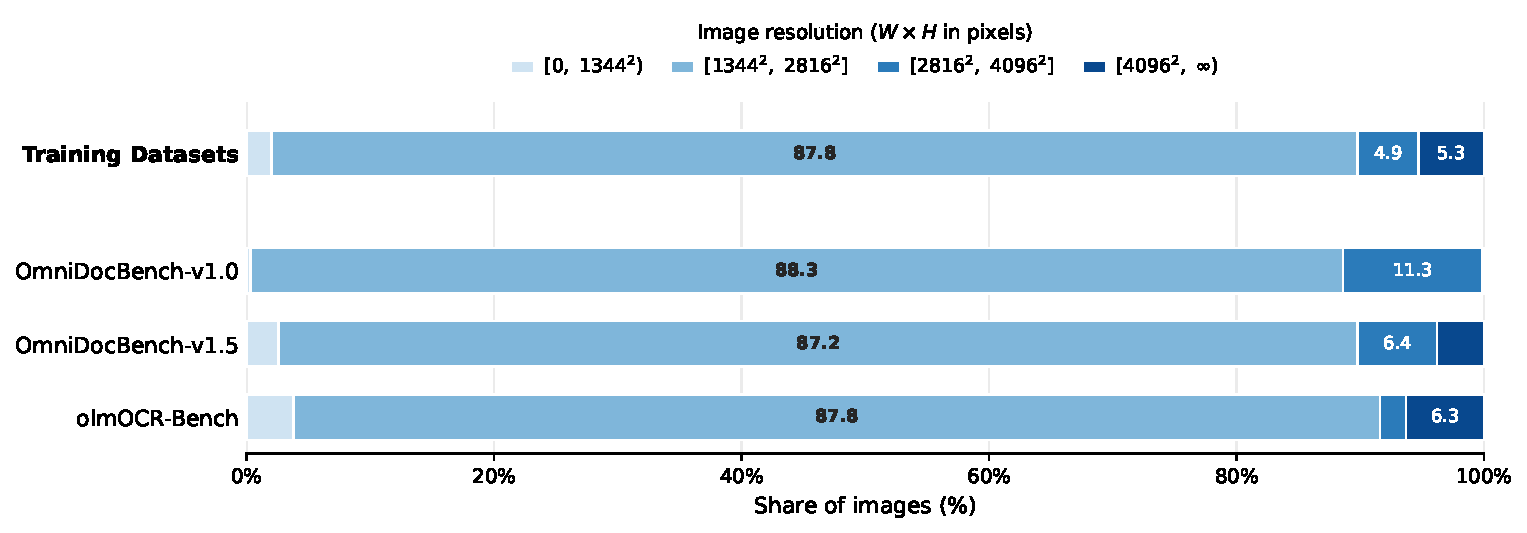
\includegraphics[width=\textwidth]{figures/resolution_distribution.pdf}
    \caption{Image resolution distribution across benchmark datasets and training dataset. Across all datasets, roughly $87$--$88\%$ of images concentrate in the $[1344^2, 2816^2]$ band, and the training distribution closely aligns with the three evaluation benchmarks.}
    \label{fig:resolution_distribution}
\end{figure*}

We ablate two design choices for our lightweight parser, the training-time image resolution and the base model. The maximum image resolution permitted during training bounds the fidelity at which fine-grained content such as small fonts, dense tables, and compact formulas is preserved, but a higher ceiling also inflates the number of visual tokens and the context length required to encode a page. We study three resolution ceilings that span this trade-off, $1344 \times 1344$, $2816 \times 2816$, and $4096 \times 4096$, each paired with a correspondingly enlarged context length of $8192$, $16384$, and $32768$ tokens. These ceilings are informed by the image-resolution distribution of our data (Figure~\ref{fig:resolution_distribution}): across the training set and the three evaluation benchmarks, roughly $87$--$88\%$ of images fall within the $[1344^2, 2816^2]$ band and the training and evaluation distributions are closely aligned, yet a non-trivial tail exceeds $2816^2$, including more than $11\%$ of OmniDocBench-v1.0. Raising the ceiling thus preserves these large pages at native resolution rather than downsampling them. The resolution sweep is conducted on the Qwen3-VL-2B~\cite{qwen3vl2025} base model, and at the highest ceiling we further replace it with the stronger Qwen3.5-2B~\cite{qwen3.5} to quantify the gain attributable to the base model alone. To isolate these factors, all configurations are trained on the same corpus of 776K Pseudo-Labeled Web Documents, differing only in the base model, the resolution ceiling, and its paired context length.

Table~\ref{tab:ablation_image_resolutions} reports the results. On olmOCR-Bench, whose verification-based protocol probes localized targets rather than full-page reconstruction, the ceiling has only a marginal effect, with the overall score rising from $78.1$ to $78.4$. The benchmarks that score full-page fidelity benefit more clearly. Raising the ceiling from $1344 \times 1344$ to $4096 \times 4096$ improves the overall score on OmniDocBench-v1.5 from $87.59$ to $88.79$ and lowers the Chinese edit distance on OmniDocBench-v1.0 (Edit-ZH) from $0.181$ to $0.157$, whereas the English edit distance (Edit-EN) is already near saturation and remains essentially unchanged ($0.129$ to $0.128$). The improvement concentrates on Chinese documents, which are typographically denser and therefore most sensitive to the detail lost when high-resolution pages are downsampled to a lower ceiling. With the ceiling fixed at $4096 \times 4096$ and a $32768$-token context, replacing the Qwen3-VL-2B base with Qwen3.5-2B brings a further consistent gain, raising olmOCR-Bench from $78.4$ to $81.4$, lifting the OmniDocBench-v1.5 overall score from $88.79$ to $89.07$, and reducing Edit-EN from $0.128$ to $0.118$, while Edit-ZH remains at $0.157$. Guided by these results, we build on the Qwen3.5-2B base model and adopt the $4096 \times 4096$ resolution ceiling with a $32768$-token context as the default training configuration.

\begin{table}[htbp]
\centering
\caption{Ablation study on image resolutions and base models for Infinity-Parser2-Flash.}
\label{tab:ablation_image_resolutions}
\small
\begin{tabular}{c@{\hspace{5pt}}c@{\hspace{5pt}}c@{\hspace{5pt}}c@{\hspace{5pt}}c@{\hspace{5pt}}c@{\hspace{5pt}}c}
\toprule
\multirow{2}{*}{\textbf{Base Model}} & \multirow{2}{*}{\textbf{Image Resolution}} & \multirow{2}{*}{\textbf{Context Length}} & \textbf{olmOCR-Bench} & \textbf{OmniDocBench-v1.5} & \multicolumn{2}{c}{\textbf{OmniDocBench-v1.0}} \\
\cmidrule(lr){4-4} \cmidrule(lr){5-5} \cmidrule(lr){6-7}
 & & & Overall $\uparrow$ & Overall $\uparrow$ & Edit-EN $\downarrow$ & Edit-ZH $\downarrow$ \\
\midrule
\multirow{3}{*}{Qwen3-VL-2B} & $1344 \times 1344$ & 8192 & 78.1 & 87.59 & 0.129 & 0.181 \\
 & $2816 \times 2816$ & 16384 & 78.3 & 87.97 & 0.128 & 0.177 \\
 & $4096 \times 4096$ & 32768 & 78.4 & 88.79 & 0.128 & \textbf{0.157} \\
\midrule
Qwen3.5-2B & $4096 \times 4096$ & 32768 & \textbf{81.4} & \textbf{89.07} & \textbf{0.118} & \textbf{0.157} \\
\bottomrule
\end{tabular}
\end{table}

\subsubsection{Ablation Study on Output Format and Reward Design}

We further ablate two coupled design choices, the output representation and the RL reward, holding the Qwen3.5-2B base, the corpus of 776K Pseudo-Labeled Web Documents, and the $4096 \times 4096$ resolution ceiling with a $32768$-token context fixed as above. We take doc2json as the target format because it serializes per-element bounding boxes and structured fields together with text, which supports layout grounding and downstream structured extraction in a single pass, whereas doc2md emits text-only Markdown that discards this spatial information. This distinction also shapes the reward, as the disentangled reward of Sec.~\ref{sec:str} depends on the bounding boxes that only doc2json provides, so on top of the doc2json SFT model we compare its textual EDS term alone against the full spatial-and-textual reward.

\begin{table}[htbp]
\centering
\caption{Ablation study on output format (doc2md versus doc2json) and RL reward design for Infinity-Parser2-Flash. On DocLayNet, `-' indicates that the doc2md output contains no layout coordinates and thus cannot be evaluated.}
\label{tab:ablation_output_format_reward}
\small
\begin{tabular}{c@{\hspace{5pt}}c@{\hspace{5pt}}c@{\hspace{5pt}}c@{\hspace{5pt}}c@{\hspace{5pt}}c@{\hspace{5pt}}c@{\hspace{5pt}}c}
\toprule
\multirow{2}{*}{\textbf{Stage}} & \multirow{2}{*}{\textbf{Task}} & \multirow{2}{*}{\textbf{Reward}} & \textbf{DocLayNet} & \textbf{olmOCR-Bench} & \textbf{OmniDocBench-v1.5} & \multicolumn{2}{c}{\textbf{OmniDocBench-v1.0}} \\
\cmidrule(lr){4-4} \cmidrule(lr){5-5} \cmidrule(lr){6-6} \cmidrule(lr){7-8}
 & & & mIoU $\uparrow$ & Overall $\uparrow$ & Overall $\uparrow$ & Edit-EN $\downarrow$ & Edit-ZH $\downarrow$ \\
\midrule
\multirow{2}{*}{SFT} & doc2md & - & - & 81.9 & 90.58 & 0.114 & 0.140 \\
 & doc2json & - & 62.94 & 81.4 & 89.07 & 0.118 & 0.157 \\
\midrule
\multirow{2}{*}{RL} & doc2json & EDS & 64.11 & 83.4 & 90.77 & 0.129 & 0.156 \\
 & doc2json & mIoU + EDS & 65.63 & 83.8 & 90.88 & 0.122 & 0.144 \\
\bottomrule
\end{tabular}
\end{table}

Table~\ref{tab:ablation_output_format_reward} reports the results. At the SFT stage the two formats reach similar text fidelity, with doc2json trailing doc2md only slightly ($81.4$ against $81.9$ on olmOCR-Bench and $89.07$ against $90.58$ on OmniDocBench-v1.5), while doc2json additionally yields $62.94$ mIoU on DocLayNet, a layout capability that doc2md cannot produce at all. We therefore apply RL to doc2json rather than doc2md, since only doc2json admits the spatial reward and produces layout output. The textual EDS reward alone already lifts doc2json to $83.4$ on olmOCR-Bench, $90.77$ on OmniDocBench-v1.5, and $64.11$ mIoU on DocLayNet, and adding the spatial mIoU term improves every metric further, reaching $65.63$ mIoU, $83.8$ on olmOCR-Bench, and $90.88$ on OmniDocBench-v1.5 while lowering the Chinese edit distance from $0.157$ to $0.144$. The spatial term thus benefits text parsing as well as layout, which indicates that accurate localization feeds back into reading order and content fidelity, a gain that a text-only doc2md model cannot obtain. The final doc2json parser surpasses the doc2md SFT baseline on both olmOCR-Bench and OmniDocBench-v1.5, adds strong layout capability, and remains comparable on the OmniDocBench-v1.0 edit distances, so we adopt doc2json output trained with the mIoU + EDS reward as the default configuration.

\subsubsection{Ablation Study on Data Curation}
\label{sec:ablation_data_curation}

To assess the data iteration flywheel (Sec.~\ref{sec:flywheel}), we track benchmark performance across its successive rounds, grouped into two phases. The metric-improvement phase (Rounds 1--3) progressively enriches document-parsing and layout-analysis data to push the core parsing metrics, whereas the capability-expansion phase (Rounds 3--5) broadens task coverage by adding element-parsing data and then reasoning and generalization data, with Round 3 as the hinge between the two. Newly curated data are appended to the cumulative corpus at every round rather than replacing it, so each round isolates the marginal contribution of the data it introduces.

\begin{table*}[htbp]
\centering
\caption{Ablation on the metric-improvement rounds (Rounds 1--3), which progressively add document-parsing and layout-analysis data.}
\label{tab:ablation_data_curation_structure}
\resizebox{0.62\textwidth}{!}{
\begin{tabular}{llcc}
\toprule
\textbf{Round} & \textbf{Cumulative training data} & \textbf{olmOCR-Bench} & \textbf{DocLayNet} \\
\midrule
Round 1 & Public \& manually-labeled data & 28.4 & 49.03 \\
Round 2 & + Pseudo-labeled web data & 83.3 & 62.48 \\
Round 3 & + Synthesized data & 85.3 & 62.31 \\
\bottomrule
\end{tabular}
}
\end{table*}

\begin{table*}[htbp]
\centering
\caption{Ablation on the capability-expansion rounds (Rounds 3--5). From the Round 3 baseline, we add element-parsing data and then reasoning and generalization data. `-' denotes no valid output before the corresponding data is added.}
\label{tab:ablation_data_curation_element_reasoning}
\resizebox{\textwidth}{!}{
\begin{tabular}{llccccccc}
\toprule
\textbf{Round} & \textbf{Configuration} & \textbf{olmOCR-Bench} & \textbf{DocLayNet} & \textbf{UniMERNet} & \textbf{Chart2Table} & \textbf{CoSyn-Chemical} & \textbf{InfoVQA} & \textbf{MMBench-EN} \\
\midrule
Round 3 & Baseline & 85.3 & 62.31 & - & 17.39 & - & 21.71 & 62.11 \\
Round 4 & + element parsing datasets & 84.7 & 61.71 & 96.70 & 79.69 & 63.54 & 52.98 & 69.07 \\
Round 5 & + reasoning and generalization datasets & 84.3 & 60.81 & 96.79 & 79.96 & 64.25 & 75.73 & 77.66 \\
\bottomrule
\end{tabular}
}
\end{table*}

\textbf{Metric-improvement rounds.} Table~\ref{tab:ablation_data_curation_structure} reports the first phase. Trained only on public and manually-labeled data, Round 1 attains 28.4 on olmOCR-Bench~\cite{poznanski2025olmocr} and 49.03 on DocLayNet~\cite{pfitzmann2022doclaynet}, reflecting the limited scale and coverage of readily available supervision. Incorporating the pseudo-labeled web data mined and annotated by the flywheel (Round 2) produces the dominant gain, lifting olmOCR-Bench by 54.9 points to 83.3 and DocLayNet by 13.45 points to 62.48, which confirms that large-scale, weakness-targeted mining of real documents with expert-model annotation is the principal driver of core parsing accuracy. Adding synthesized documents (Round 3) yields a further 2.0-point improvement on olmOCR-Bench to 85.3 and leaves DocLayNet essentially unchanged (62.31), a modest headline effect consistent with synthesis targeting the rare layouts and long-tail elements that aggregate benchmarks under-represent.

\textbf{Capability-expansion rounds.} Table~\ref{tab:ablation_data_curation_element_reasoning} reports the second phase, starting from the Round 3 model. This baseline parses documents and analyzes layouts well (85.3 and 62.31) but lacks element-level and reasoning competence: it yields no valid output on UniMERNet~\cite{wang2024unimernet} or CoSyn-Chemical, scores only 17.39 on Chart2Table, and remains weak on InfoVQA~\cite{infovqa} (21.71) and MMBench-EN~\cite{liu2024mmbench} (62.11). Adding element-parsing data (Round 4) unlocks these capabilities from near-zero baselines, reaching 96.70 on UniMERNet and 63.54 on CoSyn-Chemical, raising Chart2Table more than fourfold to 79.69, and transferring to document-centric understanding (InfoVQA 52.98, MMBench-EN 69.07). Adding reasoning and generalization data (Round 5) then raises InfoVQA to 75.73 and MMBench-EN to 77.66 while element-parsing scores hold steady. Crucially, this expansion costs only 1.0 point on olmOCR-Bench (85.3 to 84.3) and 1.5 on DocLayNet (62.31 to 60.81), a minor trade-off under multi-task generalization that is far outweighed by the breadth of capabilities gained.

The two-phase progression validates the flywheel end to end. Each capability emerges precisely when its targeted data enters the corpus and is retained as later rounds add new objectives, so the pipeline first drives the core parsing metrics to a strong level through large-scale real-document mining and synthesis, then broadens Infinity-Parser2 into a general document parser covering formulas, charts, chemical formulas, and document reasoning, with negligible regression on its original strengths.

\subsubsection{Ablation Study on Training Strategies}

We first compare supervised fine-tuning (SFT) against the pretrained baseline. As shown in Table~\ref{tab:ablation_training_strategies}, SFT delivers large and consistent gains across both model sizes. For Infinity-Parser2-Flash, it raises olmOCR-Bench from $77.2$ to $85.5$, DocLayNet from $23.08$ to $63.29$, CoSyn-Chemical from $41.48$ to $65.48$, and Chart2Table from $78.70$ to $80.30$, while UniMERNet, InfoVQA, and MMBench-EN also rise to $96.75$, $74.94$, and $75.68$. For Infinity-Parser2-Pro, SFT lifts olmOCR-Bench from $69.8$ to $86.7$, DocLayNet from $53.62$ to $64.41$, and Chart2Table from $85.20$ to $88.43$, with only a modest drop on CoSyn-Chemical ($73.19$ to $71.17$) and an essentially flat MMBench-EN ($85.74$ to $85.65$). These results confirm that task-specific fine-tuning is essential for document parsing. Within SFT, opening the vision encoder rather than freezing it further improves document-centric parsing on Infinity-Parser2-Flash (olmOCR-Bench $84.3$ to $85.5$, DocLayNet $60.81$ to $63.29$) at a modest cost on general understanding (MMBench-EN $77.66$ to $75.68$), so we adopt the open-encoder configuration as the SFT default.

Building on the open-encoder SFT model, we then evaluate multi-task reinforcement learning (RL). For Infinity-Parser2-Flash, RL improves most benchmarks over SFT, lifting olmOCR-Bench to $86.0$, DocLayNet to $64.97$, and Chart2Table to $80.49$, and it recovers and surpasses the general multimodal performance lost during SFT, with InfoVQA and MMBench-EN rising to $75.94$ and $77.92$. The two exceptions are CoSyn-Chemical, which falls from $65.48$ to $63.34$, and a marginal decline on UniMERNet ($96.75$ to $96.51$), pointing to a trade-off on the most specialized recognition tasks at the smaller scale. This specialized-task trade-off disappears for the larger Infinity-Parser2-Pro, where RL improves both UniMERNet ($97.51$ to $97.66$) and CoSyn-Chemical ($71.17$ to $73.19$) over SFT, alongside olmOCR-Bench ($86.7$ to $87.6$), DocLayNet ($64.41$ to $64.93$), InfoVQA ($86.12$ to $86.26$), and MMBench-EN ($85.65$ to $87.54$), with the only regression on Chart2Table ($88.43$ to $86.50$). The net gains across both parsing and general multimodal understanding at the two scales lead us to adopt multi-task RL as the final training stage for both model sizes.

\begin{table*}[htbp]
\centering
\caption{Ablation on training strategies, comparing SFT (frozen or open ViT) and multi-task RL across seven benchmarks. The best result within each model group is in \textbf{bold}. The baselines for Infinity-Parser2-Flash and Infinity-Parser2-Pro are Qwen3.5-2B and Qwen3.5-35B-A3B, respectively.}
\label{tab:ablation_training_strategies}
\resizebox{\textwidth}{!}{
\begin{tabular}{llccccccc}
\toprule
\textbf{Model} & \textbf{Configuration} & \textbf{olmOCR-Bench} & \textbf{DocLayNet} & \textbf{UniMERNet} & \textbf{Chart2Table} & \textbf{CoSyn-Chemical} & \textbf{InfoVQA} & \textbf{MMBench-EN} \\
\midrule
\multirow{4}{*}{Infinity-Parser2-Flash} & Baseline & 77.2 & 23.08 & 95.70 & 78.70 & 41.48 & 72.37 & 71.30 \\
 & SFT (Freeze ViT) & 84.3 & 60.81 & \textbf{96.79} & 79.96 & 64.25 & 75.73 & 77.66 \\
 & SFT (Open ViT) & 85.5 & 63.29 & 96.75 & 80.30 & \textbf{65.48} & 74.94 & 75.68 \\
 & Multi-Task RL & \textbf{86.0} & \textbf{64.97} & 96.51 & \textbf{80.49} & 63.34 & \textbf{75.94} & \textbf{77.92} \\
\midrule
\multirow{3}{*}{Infinity-Parser2-Pro} & Baseline & 69.8 & 53.62 & 97.10 & 85.20 & \textbf{73.19} & 84.51 & 85.74 \\
 & SFT (Open ViT) & 86.7 & 64.41 & 97.51 & \textbf{88.43} & 71.17 & 86.12 & 85.65 \\
 & Multi-Task RL & \textbf{87.6} & \textbf{64.93} & \textbf{97.66} & 86.50 & \textbf{73.19} & \textbf{86.26} & \textbf{87.54} \\
\bottomrule
\end{tabular}
}
\end{table*}

\subsection{Inference Speed}

\begin{table}[htbp]
\centering
\small
\caption{Inference performance comparison of specialized VLMs and Infinity-Parser2 across different backends. `TP' denotes tensor-parallel, and `C' means concurrency.}
\label{tab:inference_speed}
\begin{tabular}{lccccccc}
\toprule
\textbf{Model} & \textbf{Size} & \textbf{Hardware} & \textbf{Task} & \textbf{Config} & \textbf{Tokens / Page} & \textbf{Tokens / Sec.} & \textbf{Sec. / Page} \\
\midrule
GPT-5.2 & - & API & doc2md & C=1 & 1330.49 & 35.12 & 37.51 \\
Gemini-3.1-Pro & - & API & doc2md & C=1 & 1038.08 & 93.84 & 10.73 \\
\midrule
MinerU2.5 & 1.2B & H100 & doc2md & TP=1, C=1 & 1042.11 & 296.38 & 3.45 \\
PaddleOCR-VL-1.5 & 0.9B & H100 & doc2md & TP=1, C=1 & 1842.04 & 700.04 & 2.48 \\
DeepSeek-OCR-2 & 3B & H100 & doc2md & TP=1, C=1 & 1056.67 & 439.67 & 2.35 \\
\midrule
\multirow{2}{*}{Infinity-Parser-7B} & \multirow{2}{*}{7B} & \multirow{2}{*}{H100} & doc2md & TP=1, C=1 & 885.22 & 114.89 & 7.44 \\
 &  &  & doc2md & TP=2, C=8 & 882.24 & 441.12 & 2.18 \\
\midrule
\multirow{2}{*}{Infinity-Parser2-Flash} & \multirow{2}{*}{2B} & \multirow{2}{*}{H100} & doc2json & TP=1, C=1 & 1510.33 & 244.30 & 6.06 \\
 & & & doc2json & TP=2, C=8 & 1546.99 & 1624.22 & 0.95 \\
\midrule
\multirow{2}{*}{Infinity-Parser2-Pro} & \multirow{2}{*}{35B-A3B} & \multirow{2}{*}{H100} & doc2json & TP=2, C=1 & 1498.72 & 173.58 & 8.48 \\
 & & & doc2json & TP=2, C=8 & 1500.48 & 703.71 & 2.13 \\
\bottomrule
\end{tabular}
\end{table}

We assess the inference efficiency of the Infinity-Parser2 family, comprising the 2B Infinity-Parser2-Flash and the 35B-A3B Infinity-Parser2-Pro, against three groups of baselines: the proprietary GPT-5.2 and Gemini-3.1-Pro APIs, the open specialized parsers MinerU2.5, PaddleOCR-VL-1.5, and DeepSeek-OCR-2, and our previous-generation Infinity-Parser-7B. All open-weight models are served with vLLM on H100 GPUs and benchmarked on an in-house set of business financial documents, with server startup overhead excluded. The external baselines are profiled under single-stream serving (TP=1, C=1), whereas the Infinity-Parser and Infinity-Parser2 models are also measured under a batched configuration (TP=2, C=8) that reflects concurrent production load. Note that Infinity-Parser2's doc2json output, which serializes bounding-box coordinates and structured fields alongside text, reaches roughly 1,510 tokens per page, compared with nearly 1,050 for doc2md models such as MinerU2.5 and DeepSeek-OCR-2. PaddleOCR-VL-1.5 emits even more, about 1,840 tokens per page, owing mainly to the styling tokens such as border and alignment in its HTML table output.

As reported in Table~\ref{tab:inference_speed}, under the batched configuration (TP=2, C=8), Infinity-Parser2-Flash reaches 1,624 tokens/sec and 0.95 sec/page despite its longer doc2json output. This represents a 3.68x throughput gain over the previous-generation Infinity-Parser-7B (441 tokens/sec, 2.18 sec/page) at the same configuration. The larger Infinity-Parser2-Pro (35B-A3B) sustains 704 tokens/sec and 2.13 sec/page under this configuration, a higher-capacity option kept efficient by its 3B active parameters. The proprietary APIs are far slower, at 10.73 sec/page (Gemini-3.1-Pro) and 37.51 sec/page (GPT-5.2), leaving them impractical for high-volume document parsing.

\subsection{Evaluation on Real-World Document Information Extraction}
% Full task definition and pipeline are in financial_extraction_appendix.tex.

To assess the practical efficacy of Infinity-Parser2 in real-world downstream applications, we evaluate it on Financial Information Extraction (FinIE), the task of transcribing the three primary financial statements in full from unstructured annual reports, capturing every line item (e.g., \textit{Total Assets}, \textit{Net Profit}) with its attributes. Financial reports mainly drawn from the stock market form a particularly demanding setting for document intelligence, owing to their frameless, complex layouts, and high density of tabular data. Because annual reports often span hundreds of pages, we adopt a modular parse-locate-extract pipeline instead of feeding entire documents to a language model. To isolate the contribution of document parsing, we fix the locator (Inf-Retriever-v1~\cite{infly-ai_2025}) and the extractor (DeepSeek-V4-Flash~\cite{deepseekai2026deepseekv4}), and vary only the parser that converts each page into structured text. The full task definition and the three-stage pipeline are detailed in Appendix~\ref{appendix:fie}.

%%% begin table %%%
\begin{table*}[htbp]
\centering
\small
\caption{Performance comparison on the Financial Information Extraction (FinIE) task. All systems share the same page locator and information extractor, and differ only in the document parser. The \textbf{best} reported result is shown in bold. Note that `*' indicates that Infinity-Parser2-Flash is further finetuned on our internal financial table parsing datasets.}
\label{tab:finie}
\resizebox{\textwidth}{!}{
\begin{tabular}{l ccc ccc ccc ccc}
\toprule
\multirow{2}{*}{\textbf{Method}} & \multicolumn{3}{c}{\textbf{Overall}} & \multicolumn{3}{c}{\textbf{Income Statement}} & \multicolumn{3}{c}{\textbf{Balance Sheet}} & \multicolumn{3}{c}{\textbf{Cash Flow Statement}} \\
\cmidrule(lr){2-4} \cmidrule(lr){5-7} \cmidrule(lr){8-10} \cmidrule(lr){11-13}
 & Precision & Recall & F1 & Precision & Recall & F1 & Precision & Recall & F1 & Precision & Recall & F1 \\
\midrule
MinerU2.5 & 91.20 & 92.10 & 91.50 & 80.90 & 84.90 & 82.60 & 96.10 & 95.00 & 95.50 & 96.70 & 96.20 & 96.50 \\
PaddleOCR-VL-1.5 & 93.07 & 94.83 & 93.73 & 86.83 & 93.10 & 89.40 & 96.13 & 95.33 & 95.67 & 96.23 & 95.93 & 96.13 \\
DeepSeek-OCR-2 & 89.77 & 91.03 & 90.23 & 80.07 & 84.87 & 82.03 & 94.10 & 93.47 & 93.73 & 95.10 & 94.73 & 94.90 \\
\midrule
Infinity-Parser2-Flash* & \textbf{95.70} & \textbf{96.05} & \textbf{95.75} & \textbf{88.55} & \textbf{91.35} & \textbf{89.50} & \textbf{99.25} & \textbf{97.55} & \textbf{98.35} & \textbf{99.40} &
  \textbf{99.20} & \textbf{99.30} \\
\bottomrule
\end{tabular}
}
\end{table*}
%%% end table %%%

Table~\ref{tab:finie} reports the end-to-end results. Infinity-Parser2-Flash*, our Flash variant further finetuned on in-house financial tables, attains the highest overall F1 of $95.75\%$ and ranks first on every reported metric. The strongest baseline is PaddleOCR-VL-1.5~\cite{cui2025paddleocr} ($93.73\%$ overall F1), followed by MinerU2.5~\cite{niu2025mineru2} ($91.50\%$) and DeepSeek-OCR-2~\cite{wei2026deepseek2} ($90.23\%$). The Income Statement is the most challenging category for every parser, with the lowest scores throughout: Infinity-Parser2-Flash* leads at $89.50\%$ F1, against $89.40\%$ for PaddleOCR-VL-1.5 and roughly $82\%$ for both MinerU2.5 and DeepSeek-OCR-2. On the more regular Balance Sheet and Cash Flow Statement it approaches near-perfect extraction, reaching $98.35\%$ and $99.30\%$ F1. Accurate extraction of these line items hinges on faithful table structure recognition: a parser must align each numerical value with its row header (the financial concept) and column header (the reporting date). Trained with a structure-aware doc2json reward (Sec.~\ref{sec:str}), Infinity-Parser2-Flash* preserves high structural fidelity in dense and frameless tables, so that the retriever locates the correct context and the extractor returns the precise value. Baseline parsers more often merge cells or break frameless tables, producing spurious associations between values and dates that propagate to the final output. These results indicate that Infinity-Parser2 not only excels on standard parsing benchmarks but also serves as a robust front end for complex, high-stakes downstream applications.
